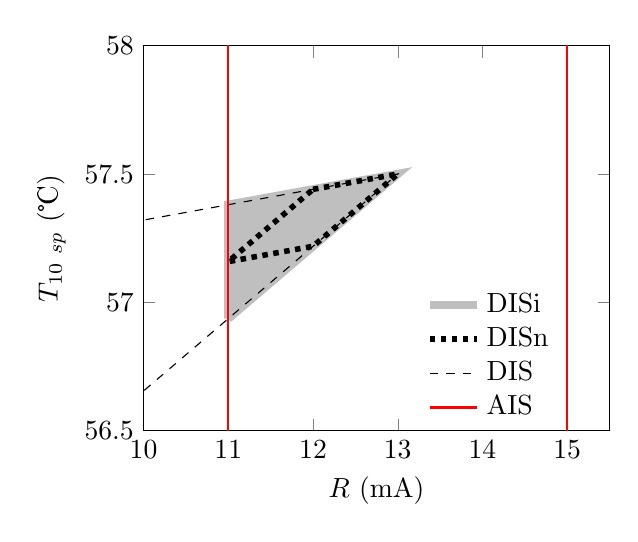
\begin{tikzpicture}
  \begin{axis}[
    width=7.5cm,
    xlabel=$R$~(mA),
    ylabel=$T_{10~sp}$~(\textcelsius),
    xmin=10,xmax=15.5,ymin=56.5,ymax=58,
 %   xtick={67,67.2,...,68.4},
 %   ytick={77.7,77.8,...,78.4},
    legend style={
      draw=none,
      at={(0.9,0.0)},
      anchor=south east,
      cells={anchor=west}}]
    %DISi
    \addplot[fill=lightgray,color=lightgray, line width=3pt] coordinates {
    (10.99999671,  56.93629251)
    (10.99999669,  57.38020814)
    (13.        ,  57.5       )
    (10.99999671,  56.93629251)
    };
    %DISn
    \addplot[color=black,dotted,line width=2pt] coordinates {
    (11.99935592,  57.44006533)
    (12.99999931,  57.49999969)
    (12.00063675,  57.21832608)
    (10.99999337,  57.15839171)
    (11.99935592,  57.44006533)
    };
    %DIS
    \addplot[color=black,dashed] coordinates {
    (-21.79048698,  55.41619479)
    ( 13.        ,  57.5       )
    (  3.61381653,  54.85447339)
    (-31.17667044,  52.77066818)
    (-21.79048698,  55.41619479)
    };
    %AIS
    \addplot[color=red,thick] coordinates {
      (11,25)
      (11,90)
      (15,90)
      (15,25)
      (11,25)
    };
    \legend{DISi,DISn,DIS,AIS}
  \end{axis}
\end{tikzpicture}
